\pgfplotsset{compat=1.15}
\usetikzlibrary{arrows}
\pagestyle{empty}
 

%<<<<<<<WARNING>>>>>>>
% PGF/Tikz doesn't support hatch filling very well
% Use PStricks for a perfect hatching export

\usetikzlibrary[patterns]
\definecolor{qqffqq}{rgb}{0,1,0}
\definecolor{ffqqtt}{rgb}{1,0,0.2}
\definecolor{qqaydv}{rgb}{0,0.6588235294117647,0.8352941176470589}
\definecolor{zzttqq}{rgb}{0.6,0.2,0}
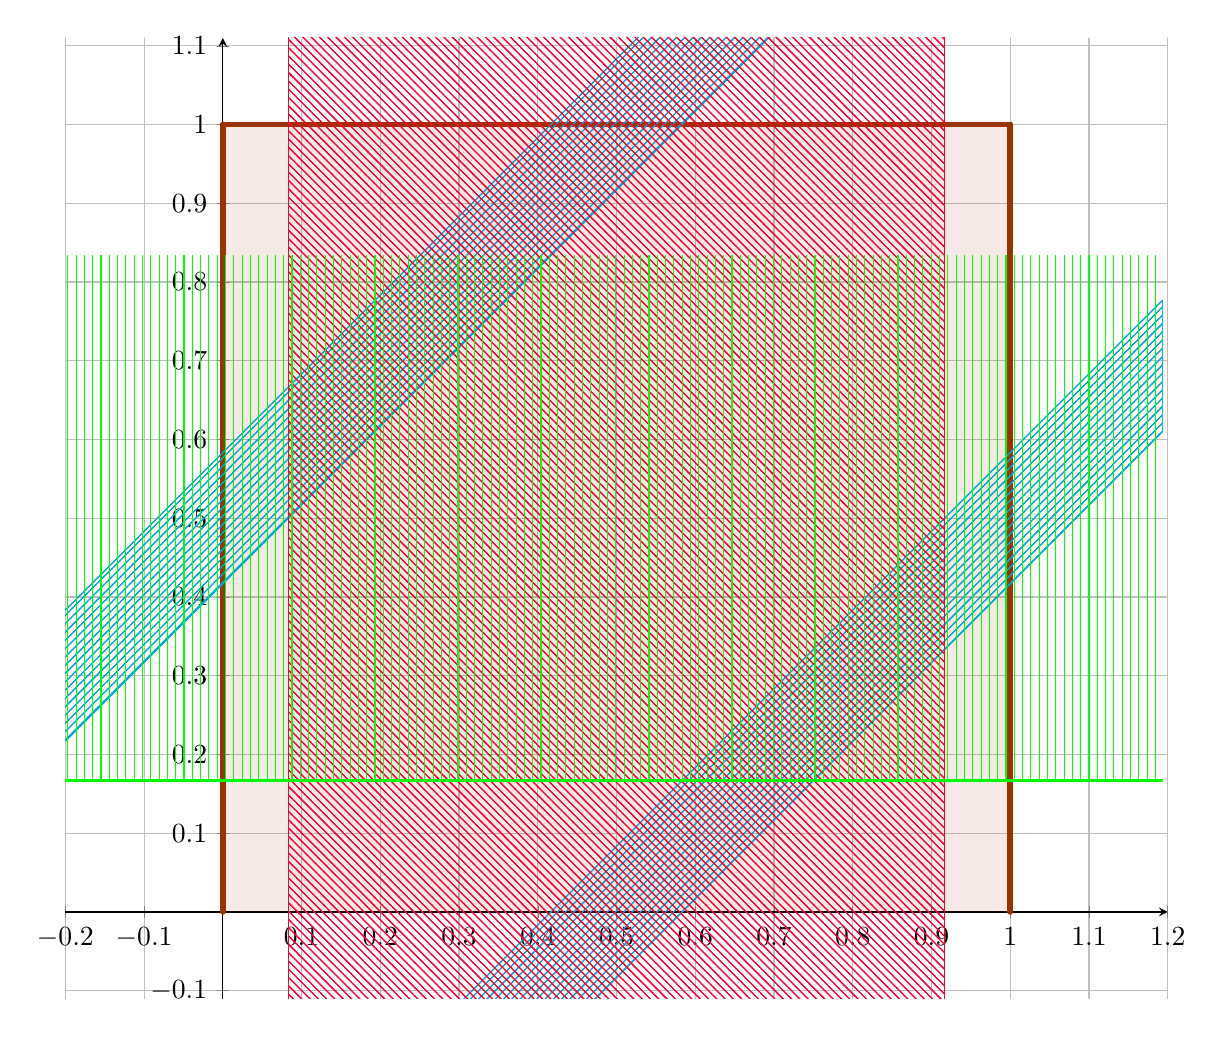
\begin{tikzpicture}[line cap=round,line join=round,>=triangle 45,x=1cm,y=1cm]
\begin{axis}[
x=10cm,y=10cm,
axis lines=middle,
ymajorgrids=true,
xmajorgrids=true,
xmin=-0.2,
xmax=1.2,
ymin=-0.11,
ymax=1.11,
xtick={-0.30000000000000004,-0.20000000000000004,...,1.3},
ytick={-0.1,0,...,1.2},]
\clip(-0.3261932561569772,-0.11133090811124503) rectangle (1.1934623633847328,1.205703962158231);
\fill[line width=2pt,color=zzttqq,fill=zzttqq,fill opacity=0.10000000149011612] (0,0) -- (1,0) -- (1,1) -- (0,1) -- cycle;
\draw [line width=2pt,color=zzttqq] (1,0)-- (1,1);
\draw [line width=2pt,color=zzttqq] (1,1)-- (0,1);
\draw [line width=2pt,color=zzttqq] (0,1)-- (0,0);
\draw[line width=0.4pt,color=qqaydv,fill=qqaydv,pattern=north east lines,pattern color=qqaydv](0.622370628824898,1.205703962158231)--(-0.3261932561569772,0.25714007717635595)--(-0.3261932561569772,0.09047341050968942)--(-0.32619325615697703,0.09047341050968957)--(0.7890372954915648,1.205703962158231);
\draw[line width=0.4pt,color=qqaydv,fill=qqaydv,pattern=north east lines,pattern color=qqaydv](1.1934623633847328,0.776795696718066)--(0.3053357585554218,-0.11133090811124488)--(0.47200242522208835,-0.11133090811124488)--(1.1934623633847328,0.6101290300513994)--(1.1934623633847328,0.776795696718066);
\draw[line width=0.4pt,color=qqaydv,fill=qqaydv,pattern=north east lines,pattern color=qqaydv](0.622370628824898,1.205703962158231)--(-0.3261932561569772,0.25714007717635595)--(-0.3261932561569772,0.09047341050968942)--(-0.32619325615697703,0.09047341050968957)--(0.7890372954915648,1.205703962158231);
\draw[line width=0.4pt,color=qqaydv,fill=qqaydv,pattern=north east lines,pattern color=qqaydv](1.1934623633847328,0.776795696718066)--(0.3053357585554218,-0.11133090811124488)--(0.47200242522208835,-0.11133090811124488)--(1.1934623633847328,0.6101290300513994)--(1.1934623633847328,0.776795696718066);
\draw[line width=0.4pt,color=ffqqtt,fill=ffqqtt,pattern=north west lines,pattern color=ffqqtt](0.08304733612311488,1.205703962158231)--(0.08304733612311488,-0.11133090811124503)--(0.9161918643806313,-0.11133090811124503)--(0.9161918643806313,1.205703962158231);
\draw[line width=0.4pt,color=ffqqtt,fill=ffqqtt,pattern=north west lines,pattern color=ffqqtt](0.08304733612311488,1.205703962158231)--(0.08304733612311488,-0.11133090811124503)--(0.9161918643806313,-0.11133090811124503)--(0.9161918643806313,1.205703962158231);
\draw[line width=1.2pt,color=qqffqq,fill=qqffqq,pattern=vertical lines,pattern color=qqffqq](-0.33952356860909744,0.8337882447440774)--(-0.33952356860909744,0.16727262213806735)--(1.206792675836853,0.16727262213806735)--(1.206792675836853,0.8337882447440774);
\draw[line width=1.2pt,color=qqffqq,fill=qqffqq,pattern=vertical lines,pattern color=qqffqq](-0.33952356860909744,0.8337882447440774)--(-0.33952356860909744,0.16727262213806735)--(1.206792675836853,0.16727262213806735)--(1.206792675836853,0.8337882447440774);
\end{axis}
\end{tikzpicture}